% !TeX TS-program = XeLaTeX
% check for outdated packages, syntax etc.
\RequirePackage[l2tabu,orthodox]{nag}

\documentclass{beamer}

\usepackage{polyglossia}
\setmainlanguage{russian}
\setotherlanguage{english}
\defaultfontfeatures{Ligatures={Common,TeX}}
\setromanfont{CMU Serif}
\setsansfont{CMU Sans Serif}
\setmonofont{CMU Typewriter Text}

\usepackage{amsmath} % math symbols, new environments and stuff
\usepackage{graphicx}
\usepackage{caption}
\usepackage{tabu}
\usepackage{tikz} % for TiKZ

\beamertemplatenavigationsymbolsempty

\setbeamerfont{page number in head/foot}{size=\large}
\setbeamertemplate{footline}[frame number]

\usetikzlibrary{positioning}
\pgfmathsetmacro{\mylinesep}{0.2cm}
\tikzset{
  bitbox/.style={
    draw,
    inner sep=2,
    outer sep=0,
    minimum height=\heightof{ABC}+2*2*1mm,
    align=center
  }
}

\hypersetup{pdfstartview={Fit}}

\title[ВКР]{Выпускная квалификационная работа бакалавра на тему}
\subtitle{``Разработка алгоритма сжатия изображений, формата для хранения и сопутствующих утилит''}
\author{Студент: {Амиантов Николай Ильич, ИУ7-82}\\Руководитель: {Рудаков Игорь Владимирович}}
\date{}

\begin{document}

\frame{\titlepage}

\begin{frame}
\frametitle{Постановка задачи}

Исходное изображение необходимо преобразовать в другое представление меньшего
размера с сохранением вида, но с потерями качества.

\begin{columns}[T]
  \begin{column}{0.45\textwidth}
    \begin{figure}
      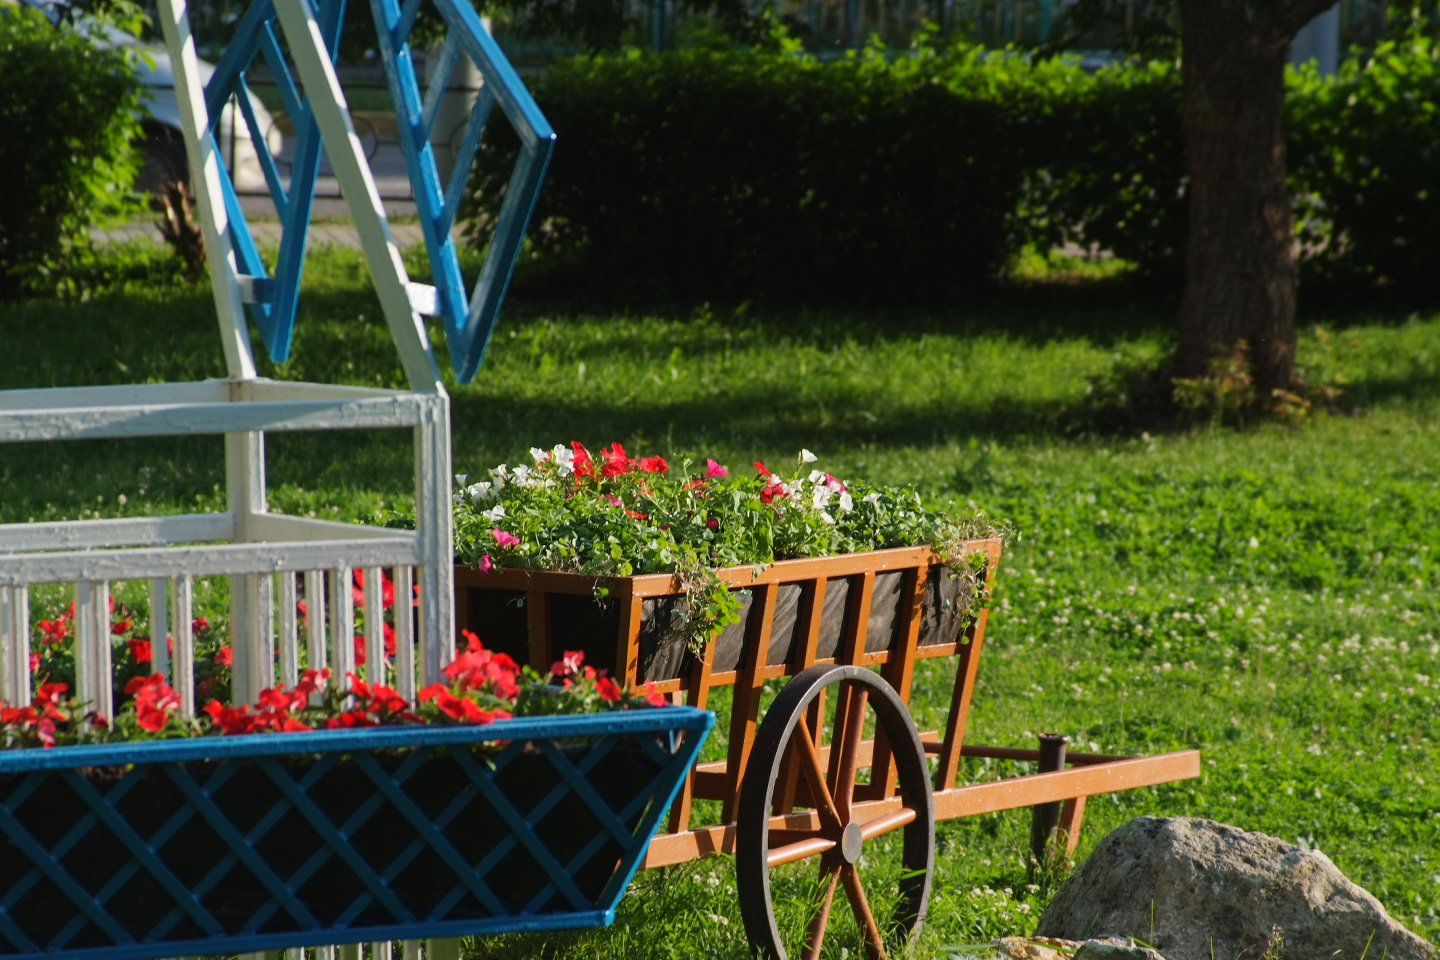
\includegraphics[width=\textwidth]{img/task}
      \caption{Оригинал}
    \end{figure}
  \end{column}

  \begin{column}{0.45\textwidth}
    \begin{figure}
      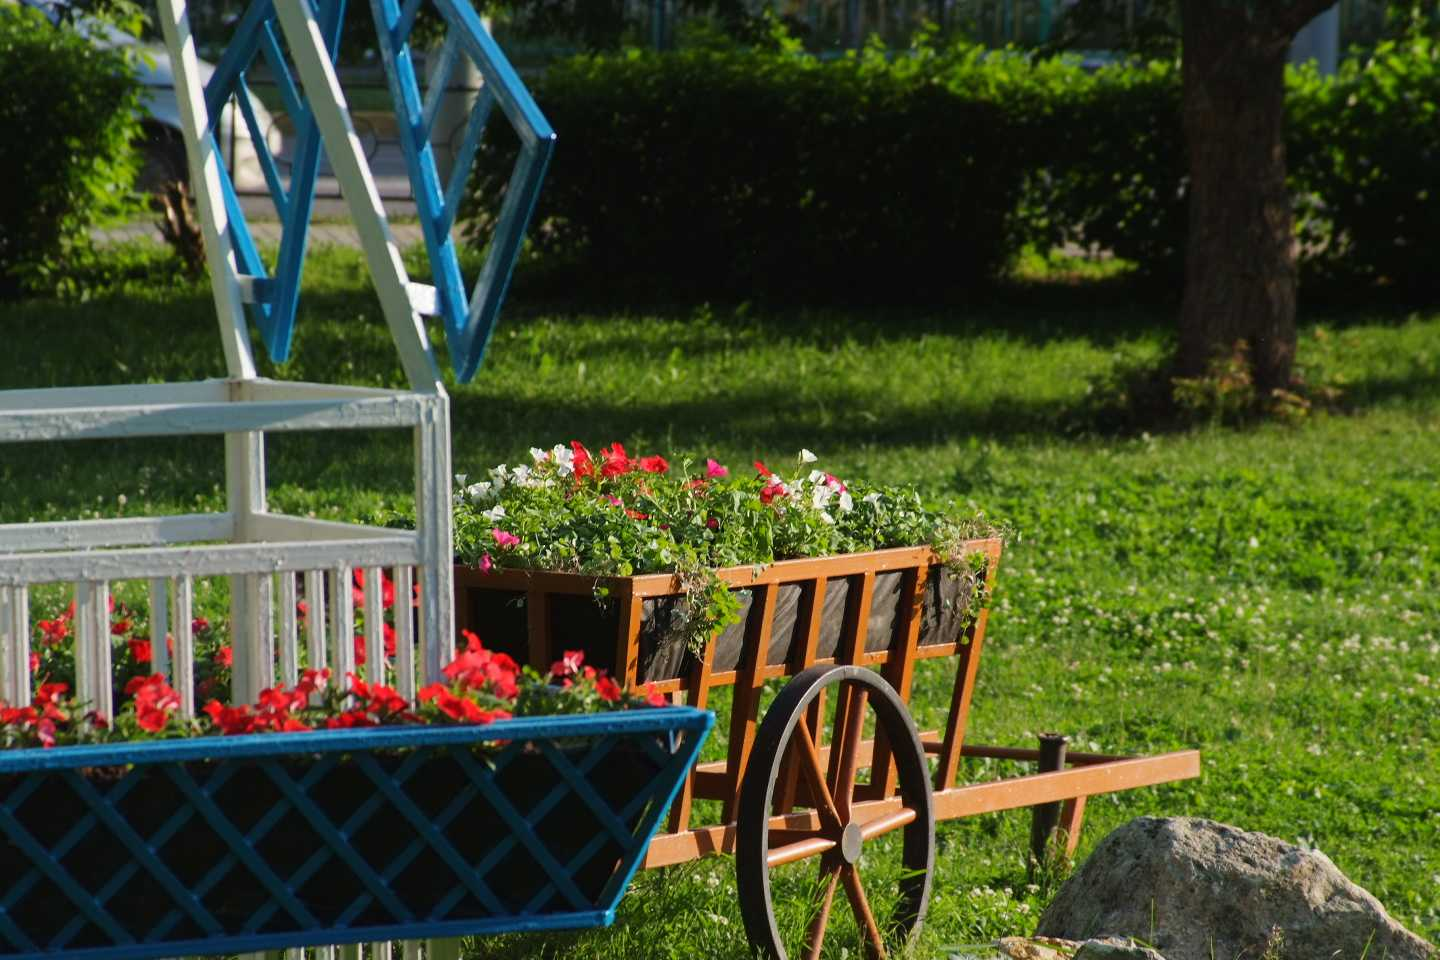
\includegraphics[width=\textwidth]{img/task_comp}
      \caption{Результат}
    \end{figure}
  \end{column}
\end{columns}

Размер результата для хороших алгоритмов сжатия должен быть существенно меньше оригинала.
\end{frame}

\begin{frame}
\frametitle{Актуальность задачи}

\begin{itemize}
\item Объёмы одиночных изображений растут
  \begin{itemize}
  \item Современные потребительские фотокамеры имеют матрицы размером 30-50 Мп;
  \item Медицинские изображения имеют огромные разрешения; используются
    специальные протоколы и форматы;
  \item Схожий рост разрешений происходит во всех областях, связанных с анализом
    изображений.
  \end{itemize}
\item Существуют и продолжают возникать банки данных изображений огромного
  объёма
  \begin{itemize}
  \item Архивы сканированных книг, журналов, газет;
  \item Медицинская история пациентов;
  \item Банки данных для проверки и обучения алгоритмов машинного зрения;
  \item Наборы астрономических и научных фотографий.
  \end{itemize}

Одним из видов изображений, которые теряют много информации от сжатия с
потерями, являются изображения с большим количеством границ.
\end{itemize}

\end{frame}

\begin{frame}
\frametitle{Цели разработки}

\begin{itemize}
\item Цель работы -- создание алгоритма сжатия изображений, сохраняющего границы
  и всплески на изображении даже при сильном сжатии.
\item Задачи:
  \begin{itemize}
  \item Изучение существующих алгоритмов сжатия, их влияния на границы в
    изображениях и причин такого влияния;
  \item Разработка базового алгоритма сжатия и обоснование его эффективности для
    задачи;
  \item Разработка формата хранения данных -- результатов работы алгоритма;
  \item Разработка и изучение различных вспомогательных алгоритмов, влияющих на
    эффективность сжатия;
  \item Проектирование структуры ПО;
  \item Реализация алгоритмов и процедур работы с разработанным форматом данных;
  \item Нахождение оптимальных настроек сжатия для различных классов изображений.
  \end{itemize}
\end{itemize}

\end{frame}

\begin{frame}
\frametitle{Существующие алгоритмы и их недостатки}

\begin{itemize}
\item Дискретное косинусное преобразование (JPEG)
  \begin{itemize}
  \item Требует деления изображения на блоки фиксированного размера;
  \item Требует задания базиса для преобразования; границы и всплески на
    изображениях сложны и могут задаваться только сложной линейной комбинацией.
  \end{itemize}
\item Дискретное вейвлет-преобразование (JPEG-2000, RemoteFX, DjVu)
  \begin{itemize}
  \item Обрабатывает изображения по двум осям -- не учитывает пространственную
    конфигурацию изображения.
  \item Может добавлять видимые ступени (новые границы).
  \item Также может удалять существующие границы (иногда хуже чем DCT).
  \end{itemize}
\item Векторное квантирование (часть MPEG-4)
  \begin{itemize}
  \item Добавляет видимые искажения на произвольных границах.
  \end{itemize}
\end{itemize}

\end{frame}

\begin{frame}
\frametitle{Сравнение артефактов сжатия}

\begin{columns}[T]
  \begin{column}{0.3\textwidth}
    \begin{figure}
      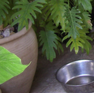
\includegraphics[width=\textwidth]{img/field/orig}
      \caption{Оригинал}
    \end{figure}
  \end{column}

  \begin{column}{0.3\textwidth}
    \begin{figure}
      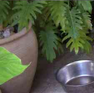
\includegraphics[width=\textwidth]{img/field/jpeg}
      \caption{DCT (JPEG)}
    \end{figure}
  \end{column}

  \begin{column}{0.3\textwidth}
    \begin{figure}
      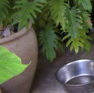
\includegraphics[width=\textwidth]{img/field/jp2k}
      \caption{DWT (JPEG-2000)}
    \end{figure}
  \end{column}

\end{columns}

Можно заметить искажения границ на сжатых изображениях.

\end{frame}

\begin{frame}
\frametitle{Вид скачков на изображениях и ошибки сжатия}

\begin{center}
  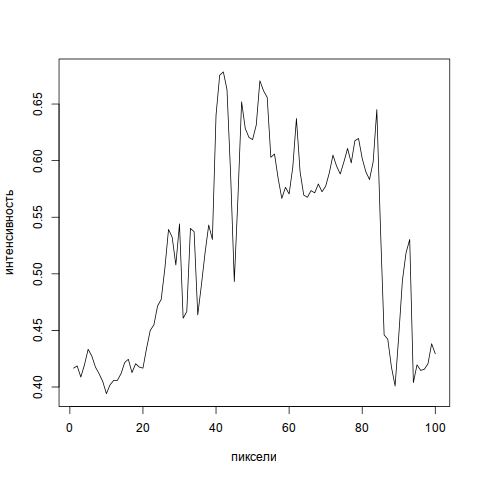
\includegraphics[height=0.4\textheight]{img/field/imageplot}
\end{center}
\begin{columns}[T]
  \begin{column}{0.45\textwidth}
    \begin{figure}
      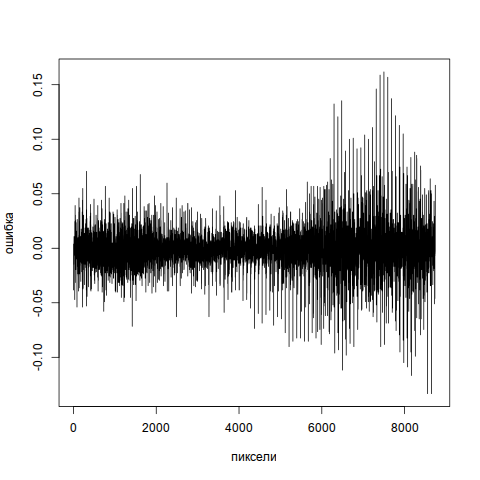
\includegraphics[height=0.3\textheight]{img/field/diffplot_jpeg}
      \caption{Ошибка для DCT}
    \end{figure}
  \end{column}

  \begin{column}{0.45\textwidth}
    \begin{figure}
      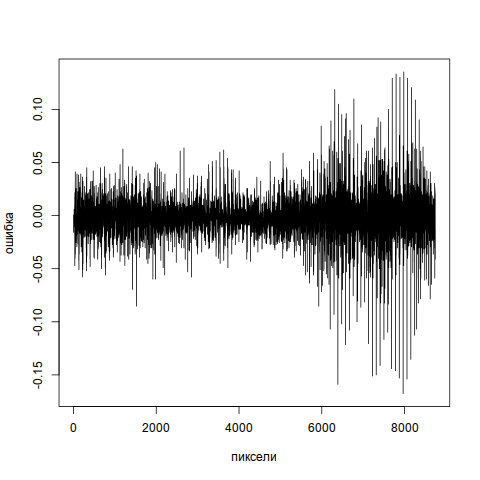
\includegraphics[height=0.3\textheight]{img/field/diffplot}
      \caption{Ошибка для DWT}
    \end{figure}
  \end{column}
\end{columns}

\end{frame}

\begin{frame}
\frametitle{Основа предложенного алгоритма}

Одним из методов, потенциально сохраняющих границы и всплески на изображении,
является понижение доступной палитры.

\begin{itemize}
  \item За основу алгоритма берётся метод квантирования интенсивностей.
  \item Используется в GIF; основной недостаток -- при увеличении размера
    палитры падает эффективность, при уменьшении -- сильно падает качество.
  \item Изображение разбивается на области.
  \item Каждая область имеет свою силу сжатия и свою палитру. Сила сжатия
    характеризуется битрейтом, размером области и количеством возможных уровней
    в палитре.
\end{itemize}

\end{frame}

\begin{frame}
\frametitle{Особенности и недостатки предложения}

\begin{itemize}
  \item При верном выборе областей для каждой возможно найти оптимальную
    малую палитру с хорошим сохранением качества;
  \item Распаковка таких изображений хорошо оптимизируется по скорости.
  \item Сложной задачей было найти оптимальный метод разбиения изображения на блоки.
  \item Ещё одна сложная задача -- способ нахождения оптимального уровня сжатия
    для блока.
\end{itemize}

\end{frame}

\begin{frame}
\frametitle{Разбиение на блоки в алгоритме}

\begin{itemize}
\item Проводились исследования способов хранения блоков изображения произвольной формы.
\item Хранить произвольные границы для каждого блока -- очень затратно.
\item Скорость такого сжатия будет крайне мала.
\end{itemize}

В итоге было решено использовать блоки прямоугольной формы. При оптимальном
способе выбора палитры это не влияет на основную особенность алгоритма --
сохранение границ. Каждый канал алгоритм хранит отдельно.

\end{frame}

\begin{frame}
\frametitle{Измерение ошибки сжатия}

\begin{itemize}
\item Алгоритм предполагает выбор силы сжатия для каждого блока отдельно.
\item Для этого мы вводим метрику, по которой можно оценивать, насколько данные
  настройки сжатия подходят для блока.
\item Введём понятие серии на блоке.
\end{itemize}

Рассмотрим блок матрицы-результата вычитания исходного канала изображения из
сжатого.
\[ \begin{bmatrix}
  a_1 & a_2 & b_1 \\
  b_2 & a_3 & b_3 \\
  b_4 & b_5 & a_6 \\
\end{bmatrix} \]
Серия -- соединённые члены блока одного знака.
\[ a_i \ge 0,\quad b_i \le 0 \]

\end{frame}

\begin{frame}
\frametitle{Введённая метрика ошибка сжатия}

Найдём серию наибольшего размера на блоке. Мы рассмотрим блоки 3х3 -- на
них можно сразу выделить серию с точкой в центре -- оптимизация по скорости.

Ошибка:
\[ e = \frac{\sum_{i=0}^n |a_i|}{n} \]

Допустимая ошибка:
\[ e_t = k \cdot max \left( \frac{\sum_{i=0}^n |a_i|}{n}, t \right) \]
, где $k$ -- коеффициент допустимости ошибки; \\
$t$ -- уровень отсечения

\end{frame}

\begin{frame}
\frametitle{Особенности метрики}

\begin{itemize}
\item Учитывает пространственную информацию
\item Ориентирована на обнаружение потери сигнала
\item В среднем не зависит от случайного шума
\end{itemize}
В результате исследования было обнаружено, что если не применять к допустимой
ошибке отсечение по минимуму, то возникают ситуации, когда допустимая ошибка
нулевая или слишком мала, и весь блок сжимается слабо.
\begin{figure}
  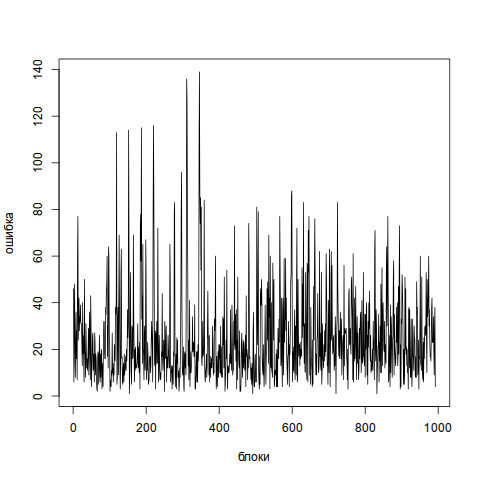
\includegraphics[height=0.3\textheight]{img/field/errplot}
  \caption{Пример расчитанной ошибки по блокам для DWT}
\end{figure}

\end{frame}

\begin{frame}
\frametitle{Блоки нескольких уровней в алгоритме}

\begin{itemize}
\item Блоки одного уровня -- недостаточно для сильного сжатия, в большом блоке
  может быть много разноцветных участков.
\item Исследовались помимо такой структуры возможные конфигурации, её усложняющие:
  \begin{itemize}
  \item Дерево уровней сжатия. Блоки вкладываются друг в друга и сопровождаются
    индексом потомка текущего узла дерева.
    \begin{itemize}
    \item Имеются затраты на указание уровня сжатия для каждого.
    \item Время сжатия растёт для каждого нового яруса.
    \end{itemize}
  \item Разбиение на блоки двух уровней; блок верхнего уровня определяет степень
    сжатия блоков нижнего уровня.
    \begin{itemize}
    \item Имеет ограничения на максимальный размер блока верхнего уровня.
    \item Экономит пространство за счёт индексов сжатия для подблоков.
    \end{itemize}
  \end{itemize}
\end{itemize}

\end{frame}

\begin{frame}
\frametitle{Нахождение оптимального размера внешнего блока}

Поскольку метрика ошибки задана нами на блоках 3х3, будем рассматривать делимые
на него размеры.

Примем 3х3 за минимальный размер блока. Мы изучили распределение размеров блоков
с одинаковым сжатием при увеличении максимального размера.

\begin{center}
  \begin{tabu} {|l|l|l|l|l|l|}
    \hline
    Размер блока & 3x3 & 6x6 & 12x12 & 18х18 & Размер \\
    \hline
    6x6 & 53\% & 47\% & 0\% & 0\% & 75K \\
    12x12 & 57\% & 17\% & 26\% & 0\% & 64K \\
    18x18 & 75\% & 22\% & 0\% & 3\% & 87K \\
    \hline
  \end{tabu}
\end{center}

Таким образом, выгодным оказывается максимальный размер блока 12х12. Чтобы
сократить размер поля индекса уровня сжатия, мы используем 4 уровня сжатия.

\end{frame}

\begin{frame}
\frametitle{Алгоритм выбора оптимального сжатия}
\centering
\includegraphics[height=0.8\textheight]{img/blockopt}
\end{frame}

\begin{frame}
\frametitle{Выбор палитры}

Алгоритмы:
\begin{itemize}
\item K-means
\item Минмакс-палитра -- минимум и максимум выборки
\item Выбор средних
\end{itemize}

\begin{center}
  \begin{tabu} {|l|l|l|l|}
    \hline
    Уровень & Средние & K-means & 2-палитра \\
    \hline
    1 & 11\% & 11\% & 4\% \\
    2 & 12\% & 16\% & 24\% \\
    3 & 45\% & 45\% & 23\% \\
    4 & 32\% & 28\% & 49\% \\
    \hline
  \end{tabu}
\end{center}

В результате экспериментов выяснилось, что для большого количества применений
K-means -- оптимальный алгоритм, однако в случае работы с палитрами размером 2
лучший визуальный результат даёт алгоритм минмакс-палитры. Также минмакс-палитра
даёт прирост скорости сжатия.

\end{frame}

\begin{frame}
\frametitle{Схема алгоритма упаковки изображения}
\centering
\includegraphics[height=0.8\textheight]{img/algorithm}
\end{frame}

\begin{frame}
\frametitle{Схема алгоритма распаковки изображения}
\centering
\includegraphics[height=0.8\textheight]{img/unpack}
\end{frame}

\begin{frame}
\frametitle{Выбор языка программирования}

\begin{itemize}
\item Библиотека для работы с форматом была написана на языке Haskell.
\item Haskell предоставляет мощную систему типов, способную отловить целые
  классы ошибок на этапе компиляции.
\item Функции в Haskell, если не нужно явно, чистые -- т.е. не содержат побочных
  эффектов и дают всегда одинаковый результат при одинаковых входных
  параметрах. Это отсекает ещё один большой класс ошибок. Итог -- если программа
  скомпилировалась верно, велика вероятность что она сразу заработает.
\item Haskell имеет ленивую модель вычислений, и мощную систему оптимизации
  кода.
\item Язык предоставляет мощнейшие средства тестирования и измерения скорости
  работы.
\item По скорости исполнения численных алгоритмов язык приближается к
  оптимизированному коду на Си.
\end{itemize}

\end{frame}

\begin{frame}
\frametitle{Структура ПО}

\begin{itemize}
\item Выбранный язык программирования поддерживает в первую очередь
  функциональную парадигму; она была выбрана для работы.
\item Программа была разбита на модули по целям использования. Алгоритмы, не
  зависящие от формата представления изображения и математические функции
  были отделены от библиотеки работы с форматом.
\item Во время разработки алгоритмов обхода и битовых преобразований применялась
  автоматическая генерация тестов для заданных свойств функций (напр.,
  идемпотентность) и профилирование.
\end{itemize}

\end{frame}

\begin{frame}
\frametitle{Структура модулей библиотеки}

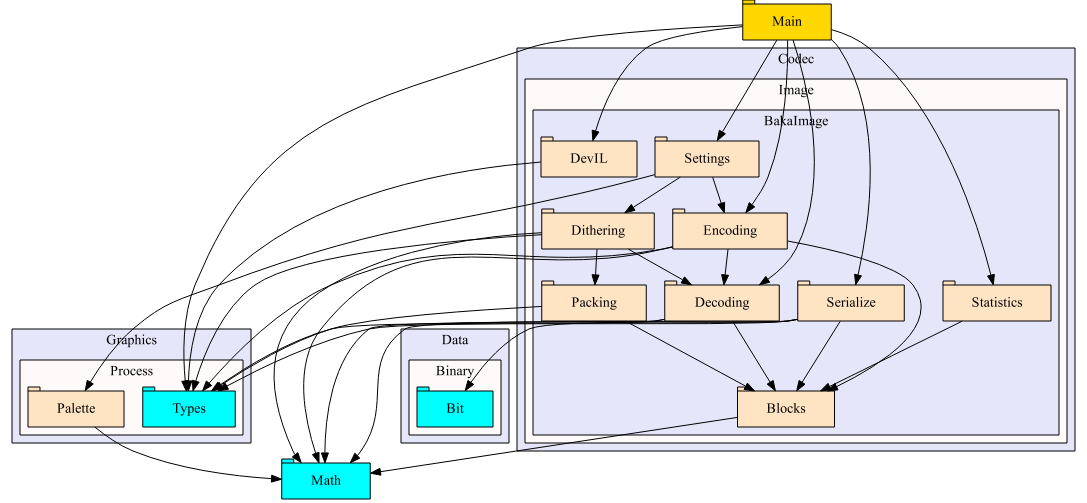
\includegraphics[width=\textwidth]{img/structure}

\end{frame}

\begin{frame}
\frametitle{Пример результатов сжатия}

\begin{columns}
  \begin{column}{0.45\textwidth}
    \begin{figure}
      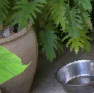
\includegraphics[width=\textwidth]{img/field/algo}
      \caption{Пример искажений при сжатии алгоритмом}
    \end{figure}
  \end{column}
  \begin{column}{0.45\textwidth}
    \begin{figure}
      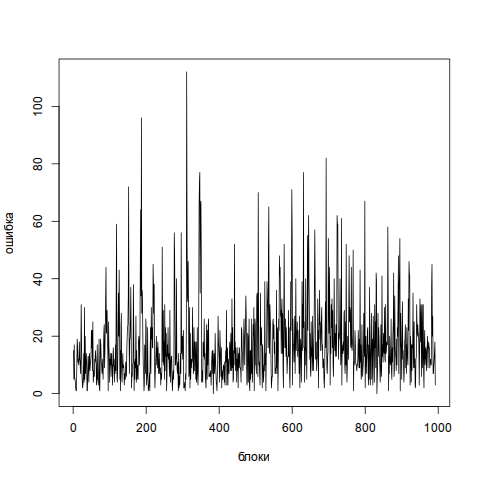
\includegraphics[width=\textwidth]{img/field/errplot_algo}
      \caption{Функция ошибки (сильное сжатие)}
    \end{figure}
  \end{column}
\end{columns}

\end{frame}

\begin{frame}
\frametitle{Выводы}

\begin{itemize}
\item Алгоритм сохраняет границы и всплески в изображении при сжатии даже при
  больших значениях $k$ и $t$.
\item Алгоритм справляется с файлами, содержащими графики или таблицы, лучше
  представленных аналогов:
  \begin{center}
    \begin{tabu} {|l|l|l|l|}
      \hline
      Формат & Средний размер файла \\
      \hline
      BMP & 260 кбайт \\
      JPEG & 49 кбайт \\
      JPEG-2000 & 41 кбайт \\
      PNG & 63 кбайт \\
      Наш алгоритм & 34 кбайт \\
      \hline
    \end{tabu}
  \end{center}
\item Алгоритм обладает большой скоростью распаковки и хорошо поддаётся
  распараллеливанию.
\end{itemize}

\end{frame}

\begin{frame}
\frametitle{Дальнейшая работа}

\begin{itemize}
\item Исследование использования других алгоритмов пост-сжатия, напр.,
  вейвлет-преобразования без потерь.
\item Изучение возможных преобразований без повторного сжатия, напр., афинных
  преобразованих.
\end{itemize}

\end{frame}

\end{document}
